Para o caso de uma função F6 com 10 variáveis, temos que:

\begin{equation}
    \begin{split}
        F(x_1 .. x_{10}) = & F6(x_1, x_2) + F6(x_2, x_3) + F6(x_3, x_4) + F6(x_4, x_5) + F6(x_5, x_6) \\
                          & F6(x_6, x_7) + F6(x_7, x_8) + F6(x_8, x_9) + F6(x_9, x_{10})
    \end{split}
\end{equation}

Portanto a seguinte configuração foi utilizada:
\begin{itemize}
	\item Representação: Representação real com 10 variáveis dentro do intervalo $[-100,100]$. Assim, o cromossomo é composto por um vetor de 10 posições.

	\item Seleção: Foi utilizados a roleta proporcional ao fitness tanto para a função $f6$
        quanto para a função $f6_{elevada}$.

    \item O Método de elitismo foi utilizado.

    \item Operadores genéticos: Para realizar o cruzamento, foi utilizado o algoritmo
    aritmético com uma taxa de cruzamento de 75\%. Também, foi utilizada mutação uniforme
    com uma taxa igual a 1\%.

	\item Critério de paragem: O critério de paragem foi 100 gerações.
\end{itemize}

Os resultados obtidos são apresentados na tabela~\ref{tab:f6_10}.

\begin{table}[htb]
	\centering
	\begin{tabular}{|c|c|c|}
		\hline
		\rowcolor[HTML]{9B9B9B}
		Teste & Média melhor indíviduo & Média população \\\hline
		1 & 7.23983 & 5.33647 \\\hline
		2 & 7.27323 & 5.29675 \\\hline
		3 & 7.32053 & 5.36799 \\\hline
		4 & 7.21803 & 5.31238 \\\hline
		5 & 7.31284 & 5.36265 \\\hline
		\textbf{Média Final} & \textbf{7.27289} & \textbf{5.33523} \\\hline	\end{tabular}
    \caption{Resultados da função $f6$ utilizando representação real, cruzamento aritmético,
    mutação uniforme e elitismo. \label{tab:f6_10}}
\end{table}

\begin{figure}[htb]
	\begin{subfigure}{.45\textwidth}
		\centering
		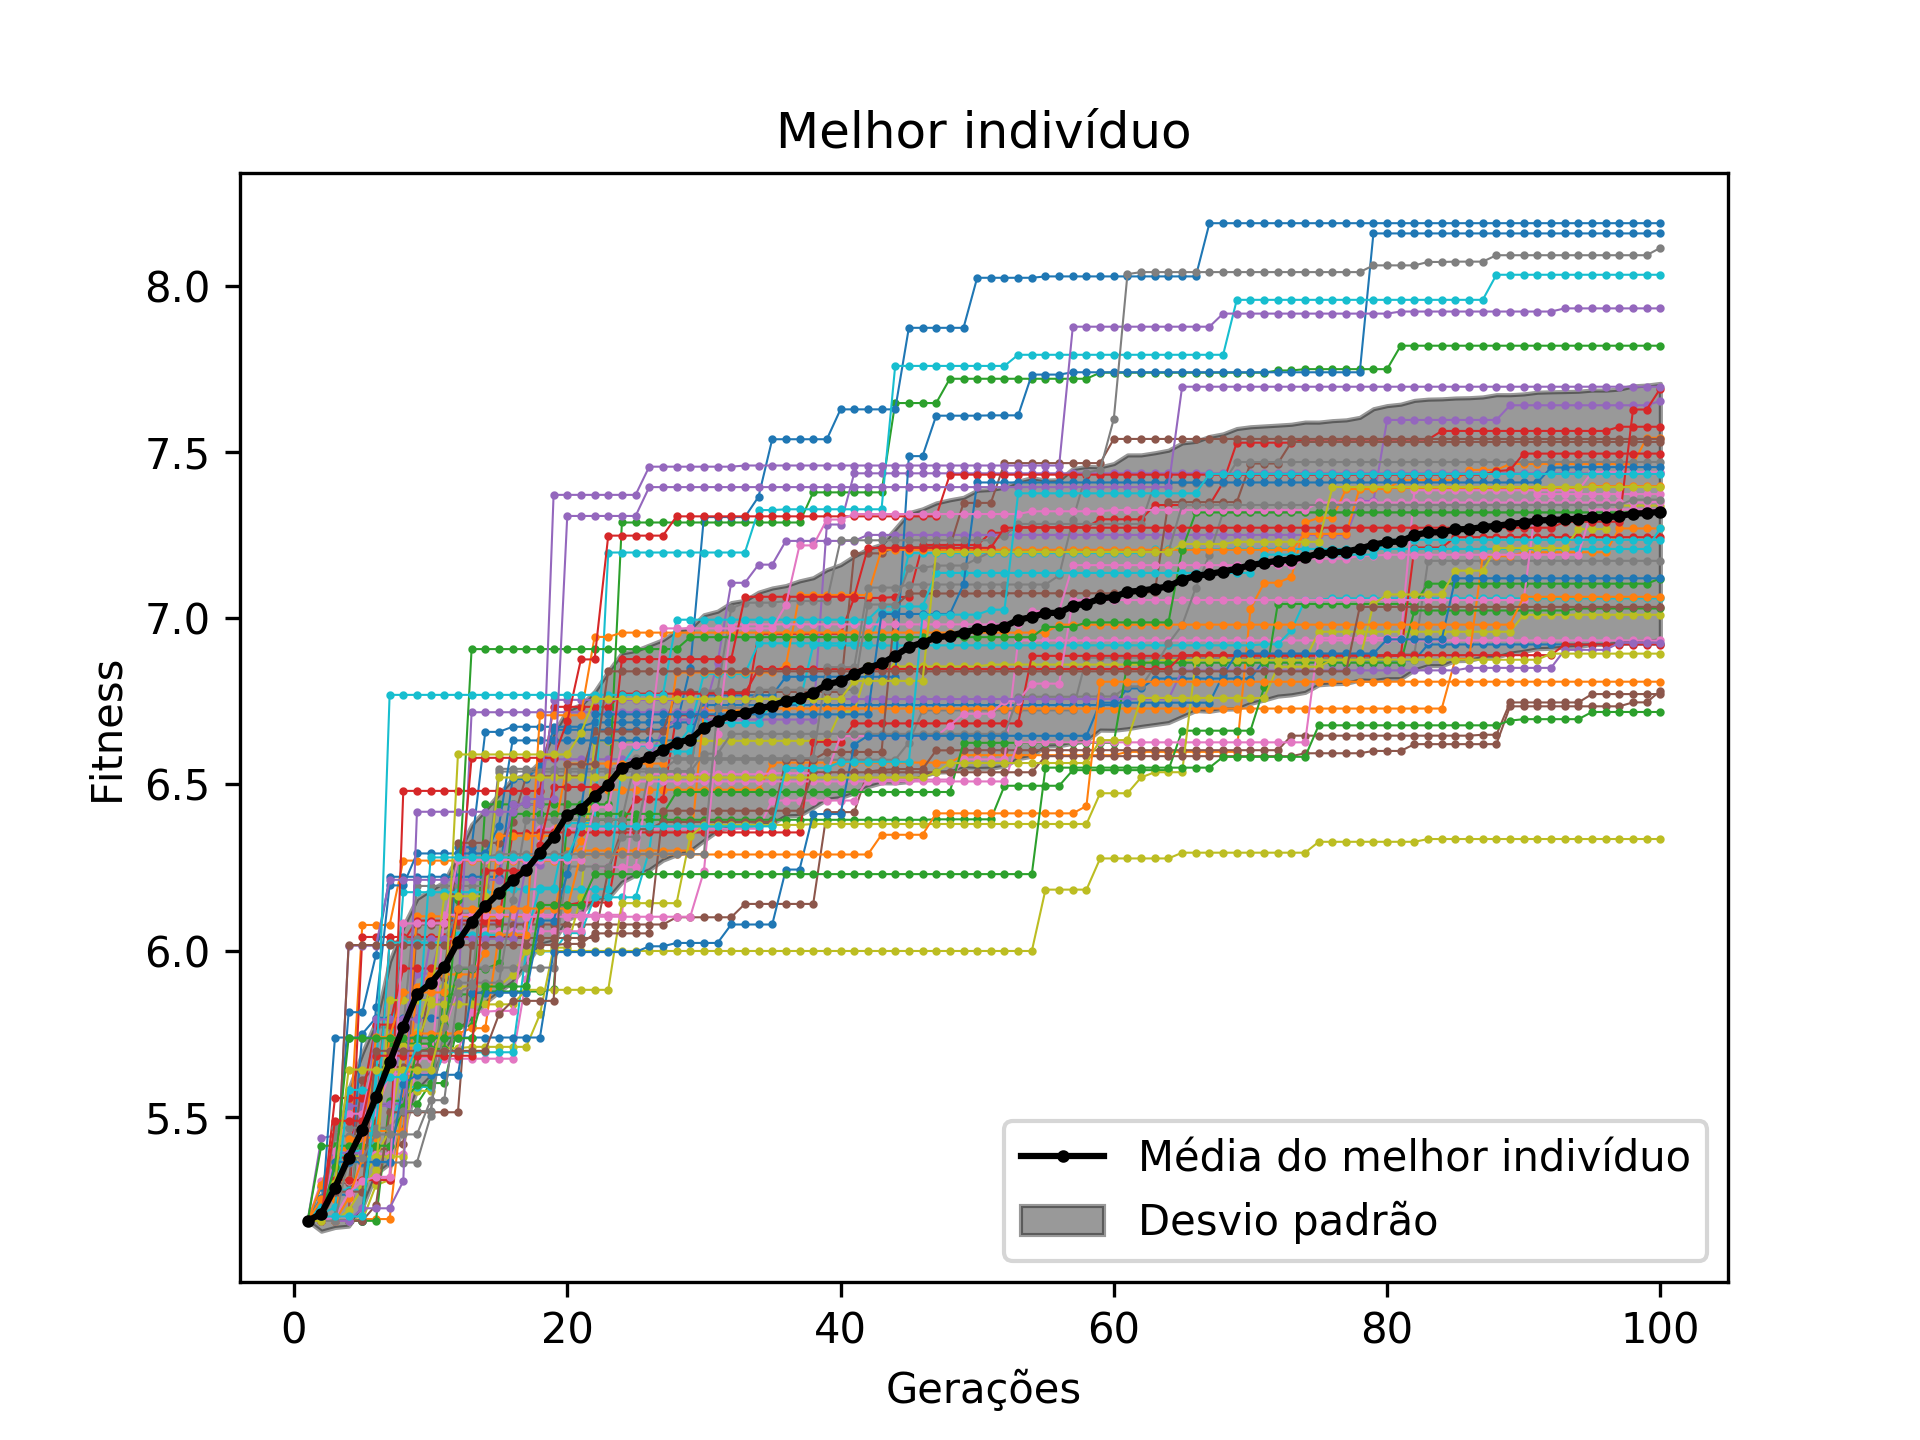
\includegraphics[width=1\textwidth]{sec-04/f6_fitness_vs_gen_best.png}
		\caption{Melhores indíviduos de todos os experimentos ao longo das gerações.
		Em preto é mostrado o comportamento médio dos 50 experimentos. }
	\end{subfigure}
	\hfill
	\begin{subfigure}{.45\textwidth}
		\centering
		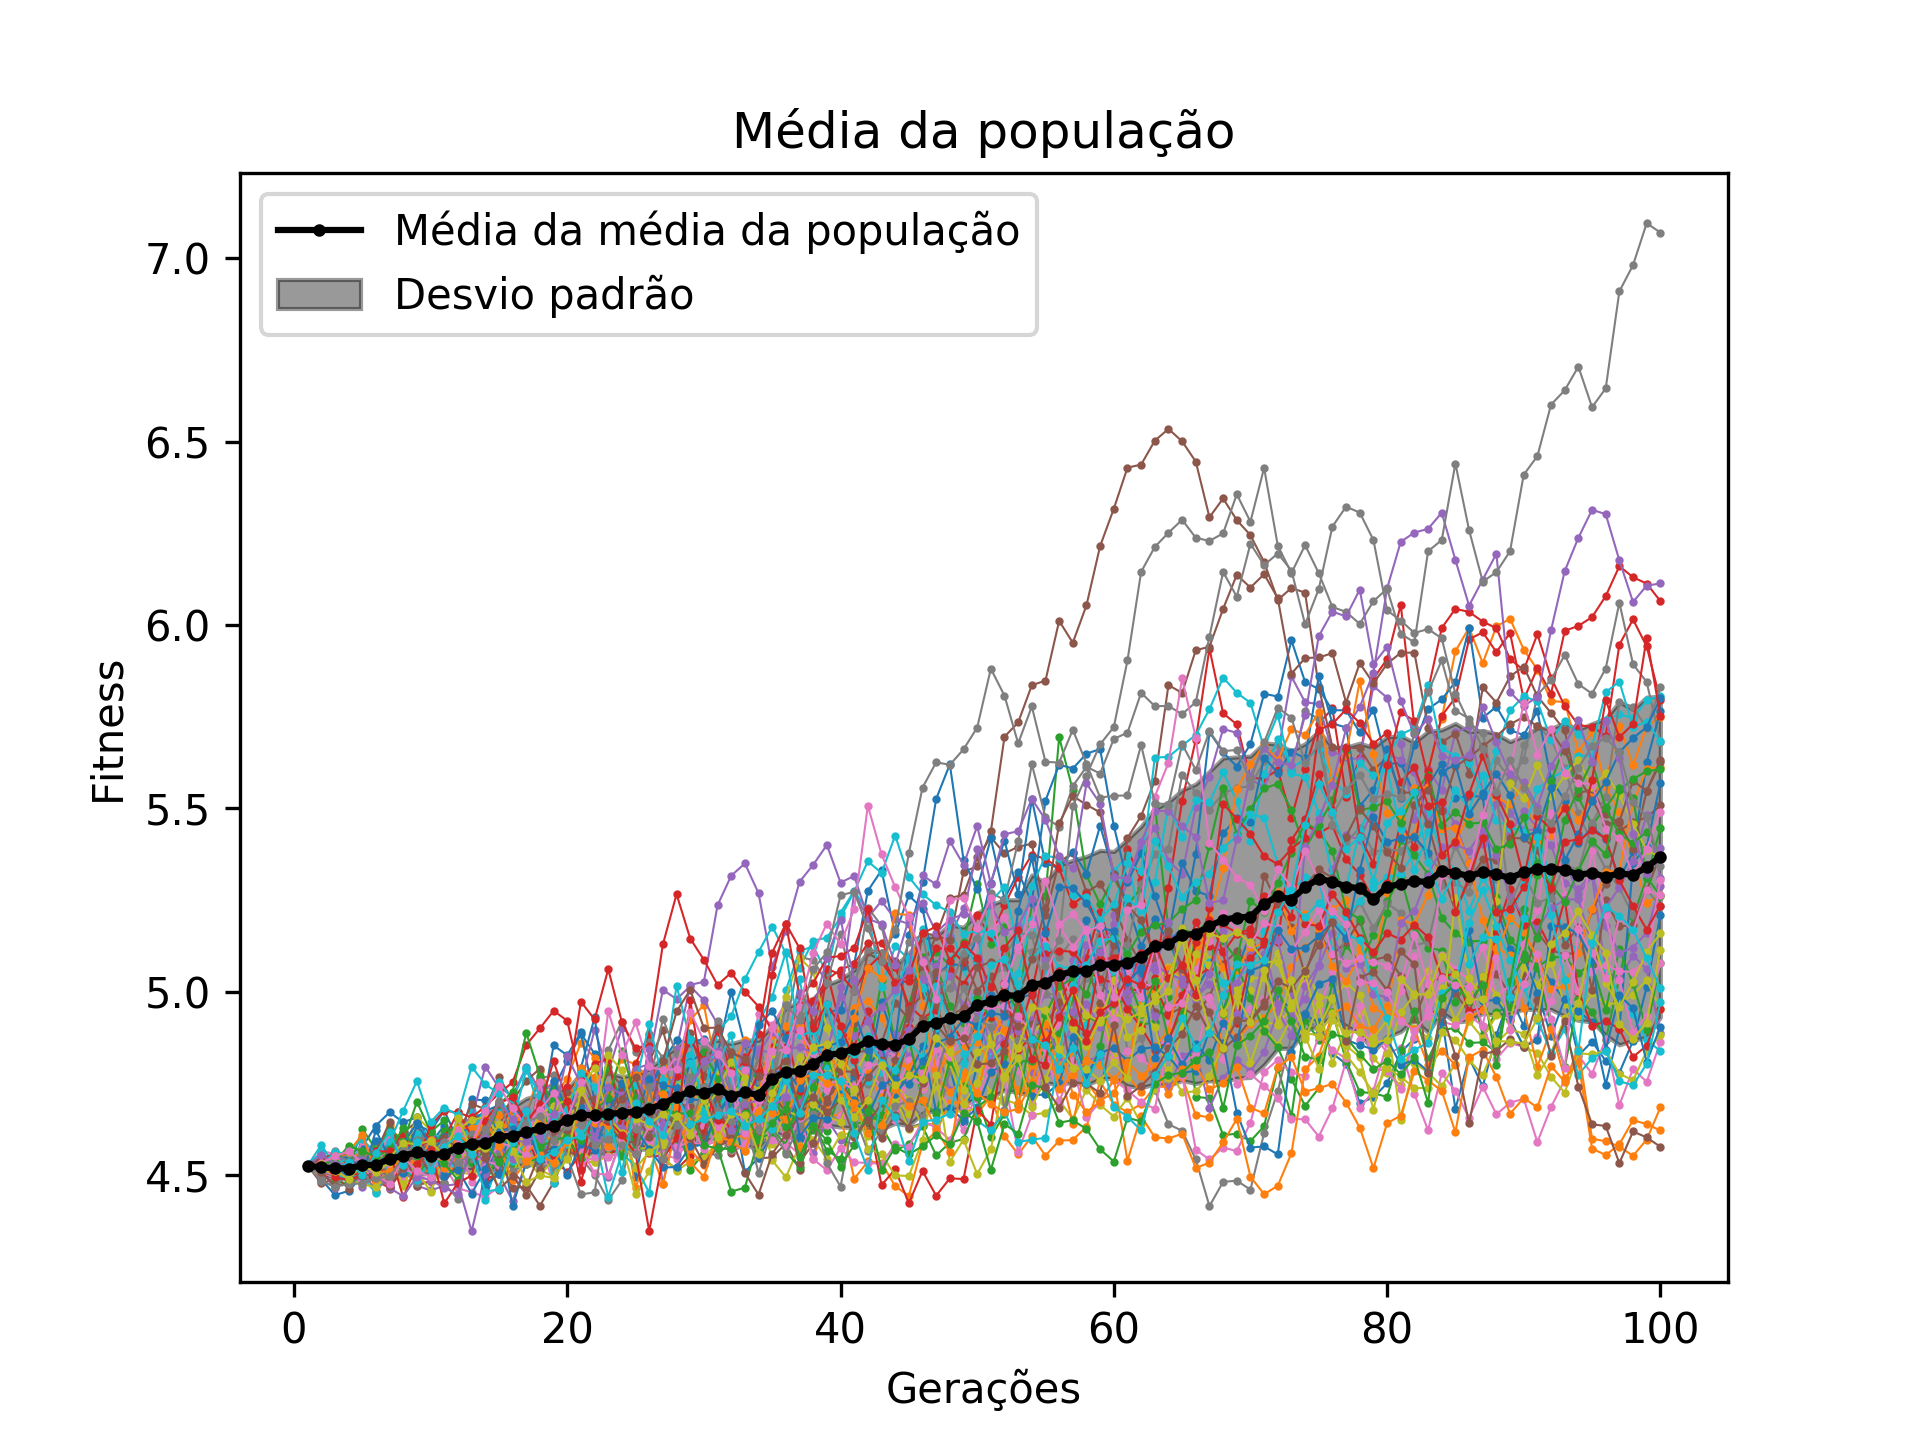
\includegraphics[width=1\textwidth]{sec-04/f6_fitness_vs_gen_pop.png}
		\caption{Média da população de todos os experimentos ao longo das gerações.
		Em preto é mostrado o comportamento médio dos 50 experimentos.}
	\end{subfigure}
	\caption{Resultados obtidos utilizando utilizando representação real, cruzamento aritmético,
    mutação uniforme e elitimo para o caso da F6 com 10 variáveis.}
\end{figure}

\begin{figure}[htb]
	\begin{subfigure}{.5\textwidth}
		\centering
		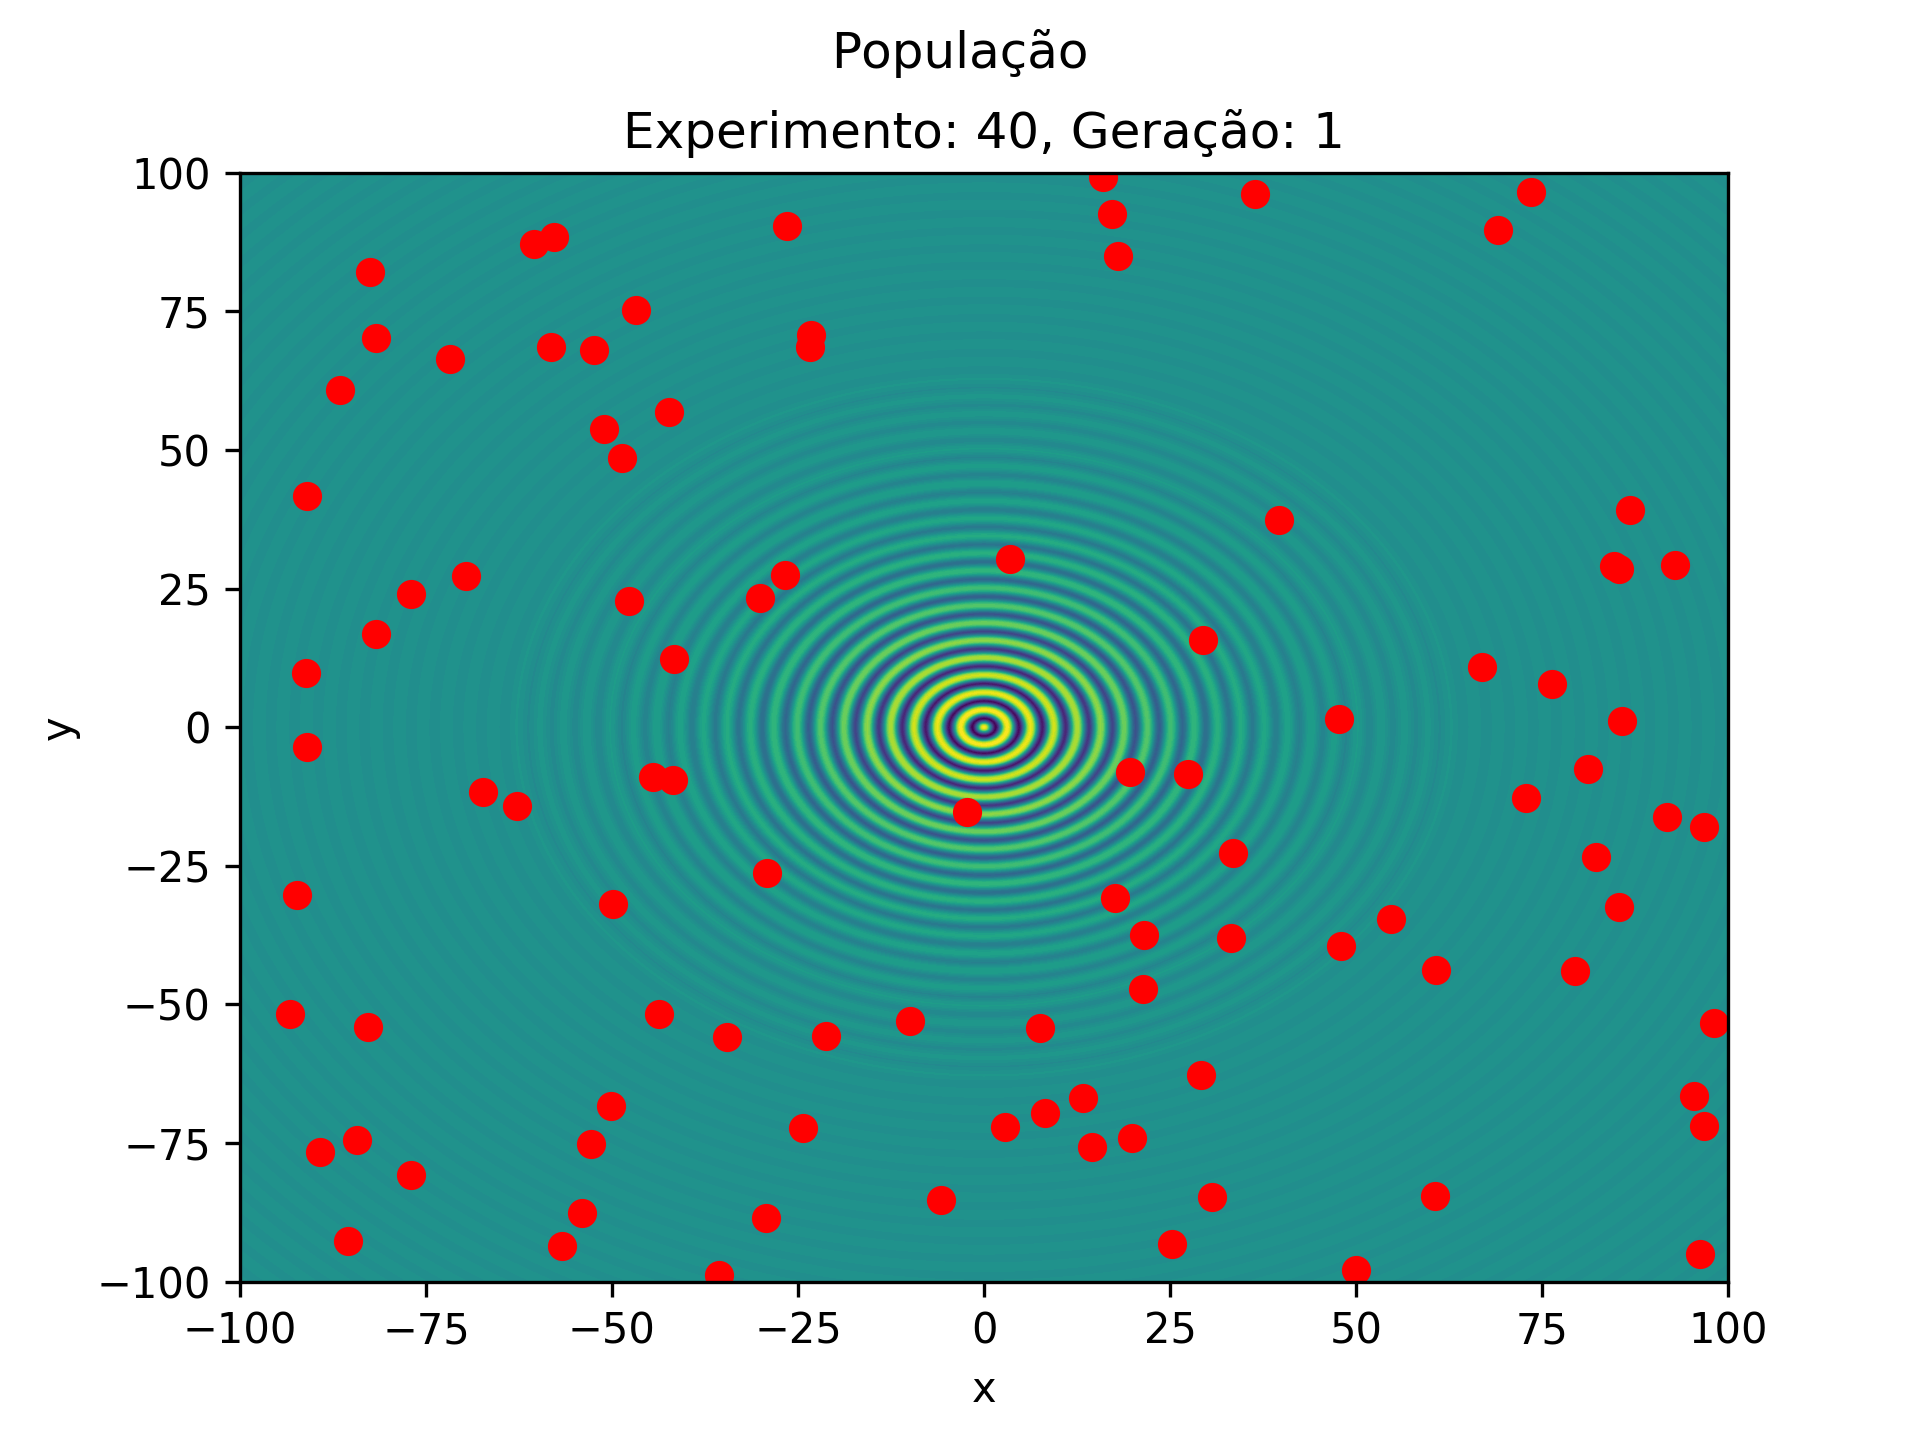
\includegraphics[width=0.9\linewidth]{sec-04/f6_population_gen_1_exp_40.png}
	  \end{subfigure}
	  \begin{subfigure}{.5\textwidth}
		\centering
		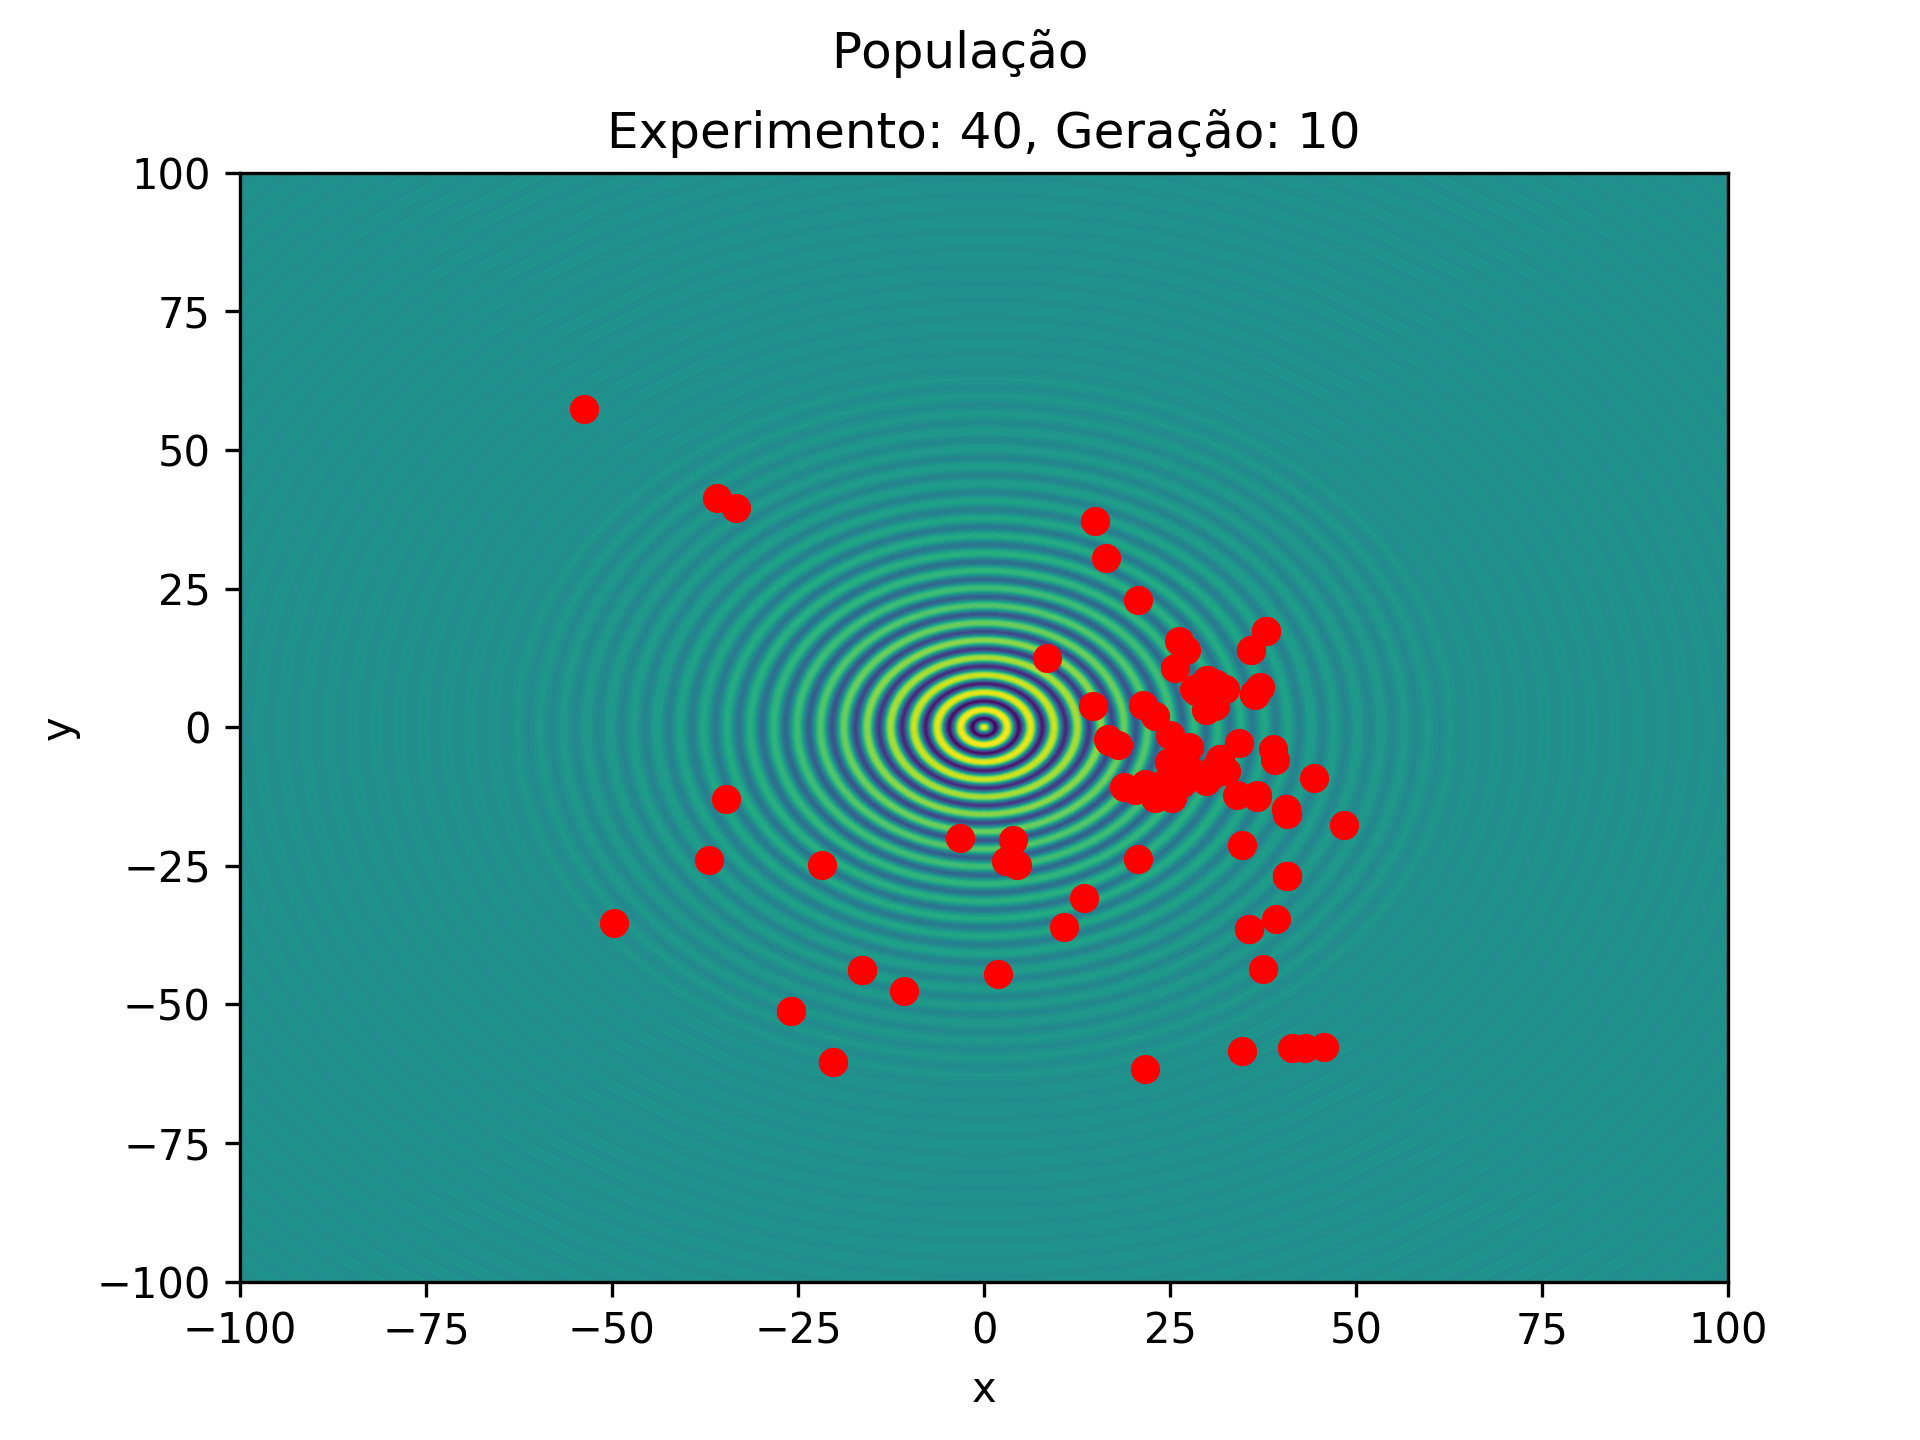
\includegraphics[width=0.9\linewidth]{sec-04/f6_population_gen_10_exp_40.png}
	  \end{subfigure}
	  \begin{subfigure}{.5\textwidth}
		\centering
		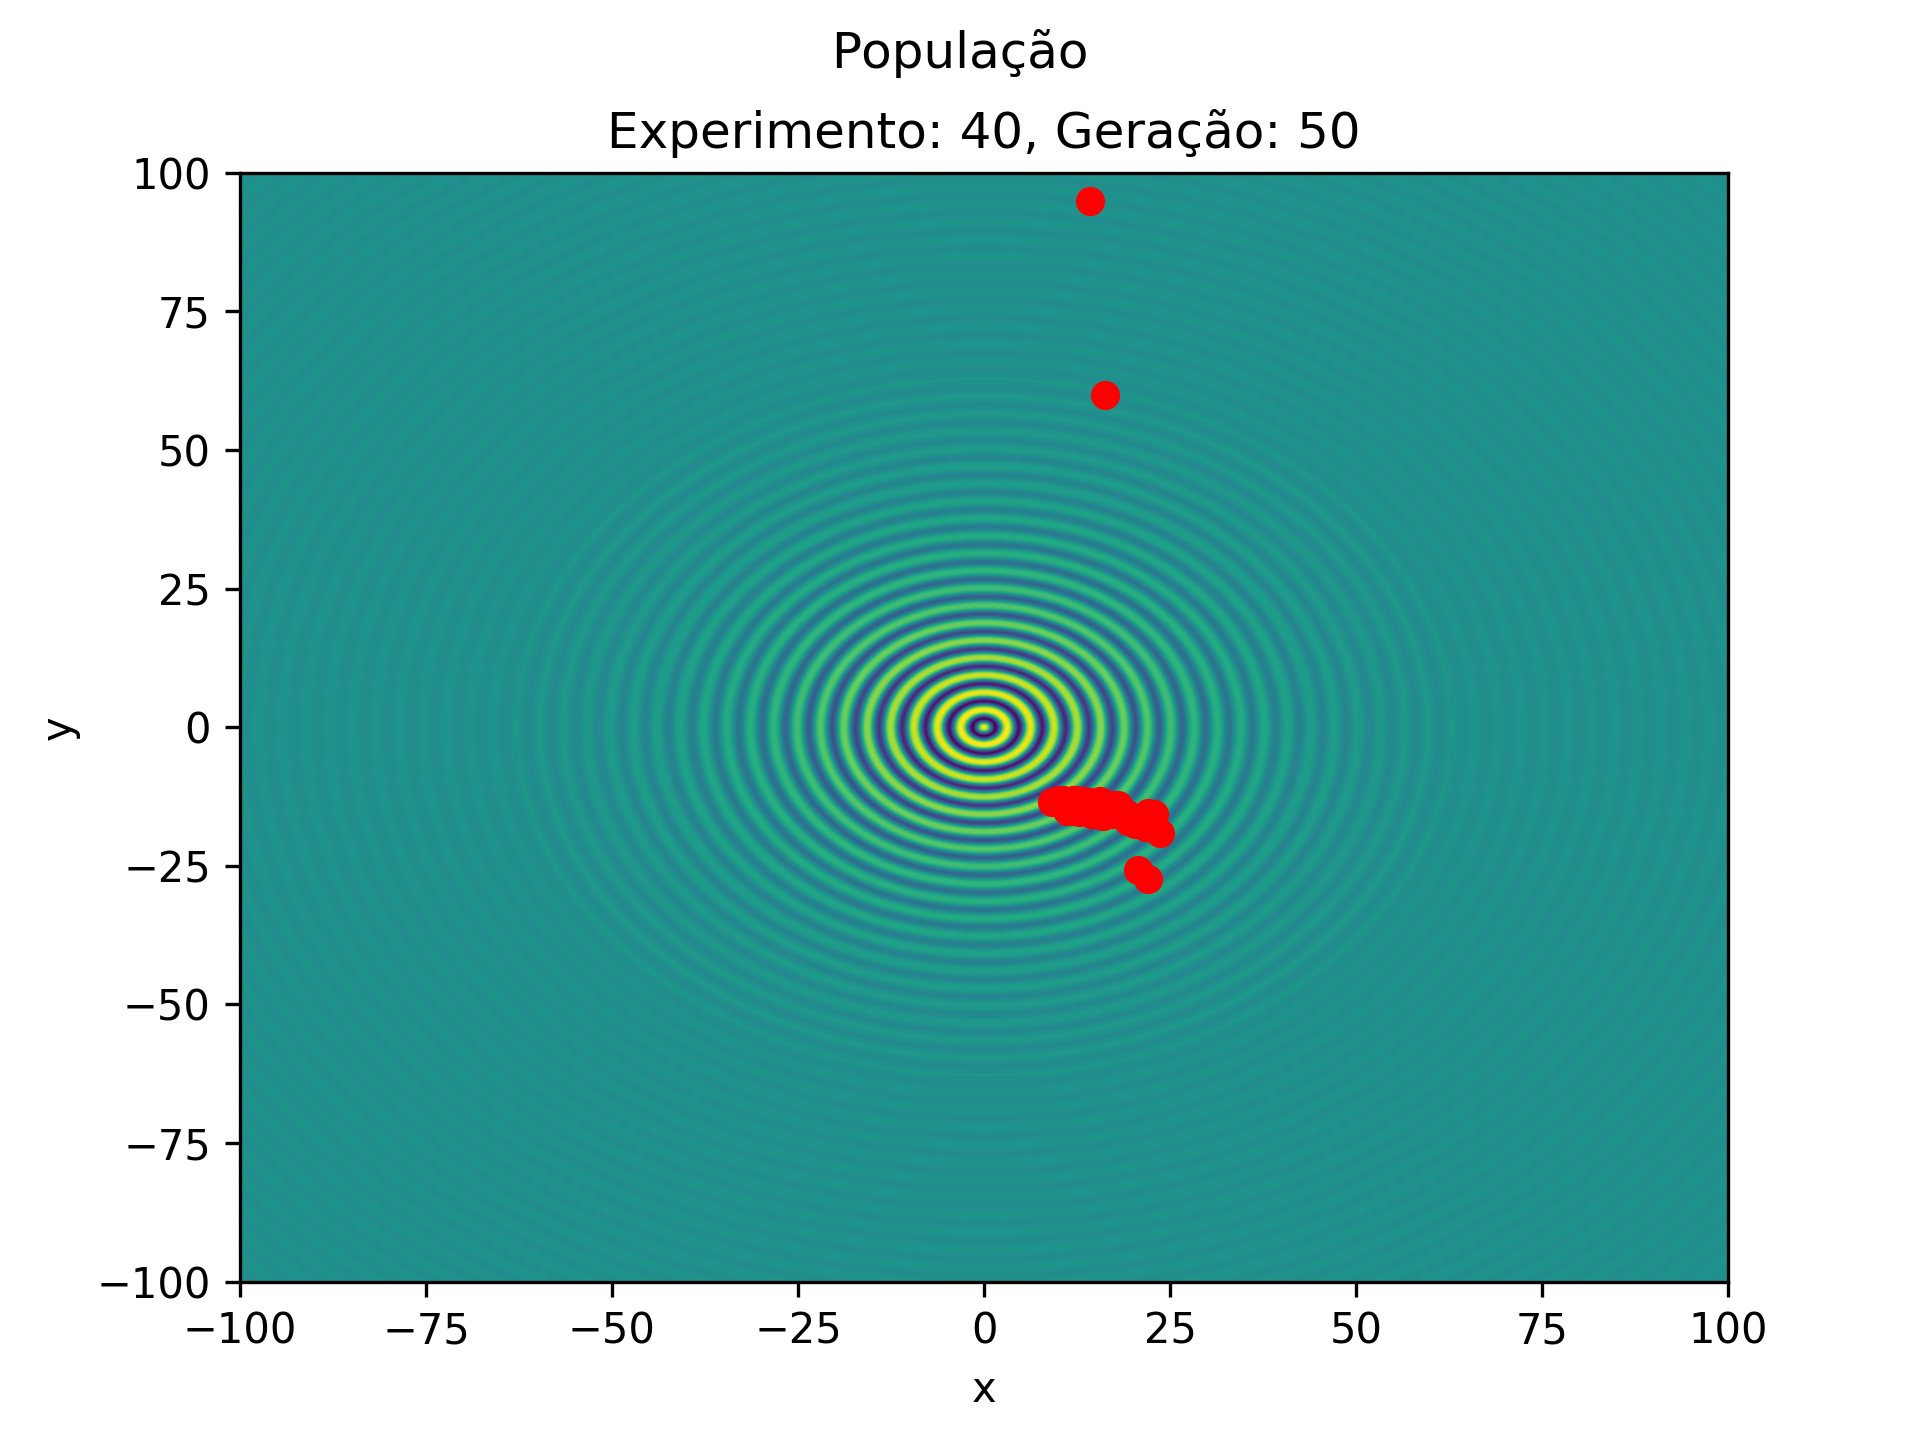
\includegraphics[width=0.9\linewidth]{sec-04/f6_population_gen_50_exp_40.png}
	  \end{subfigure}
	  \begin{subfigure}{.5\textwidth}
		\centering
		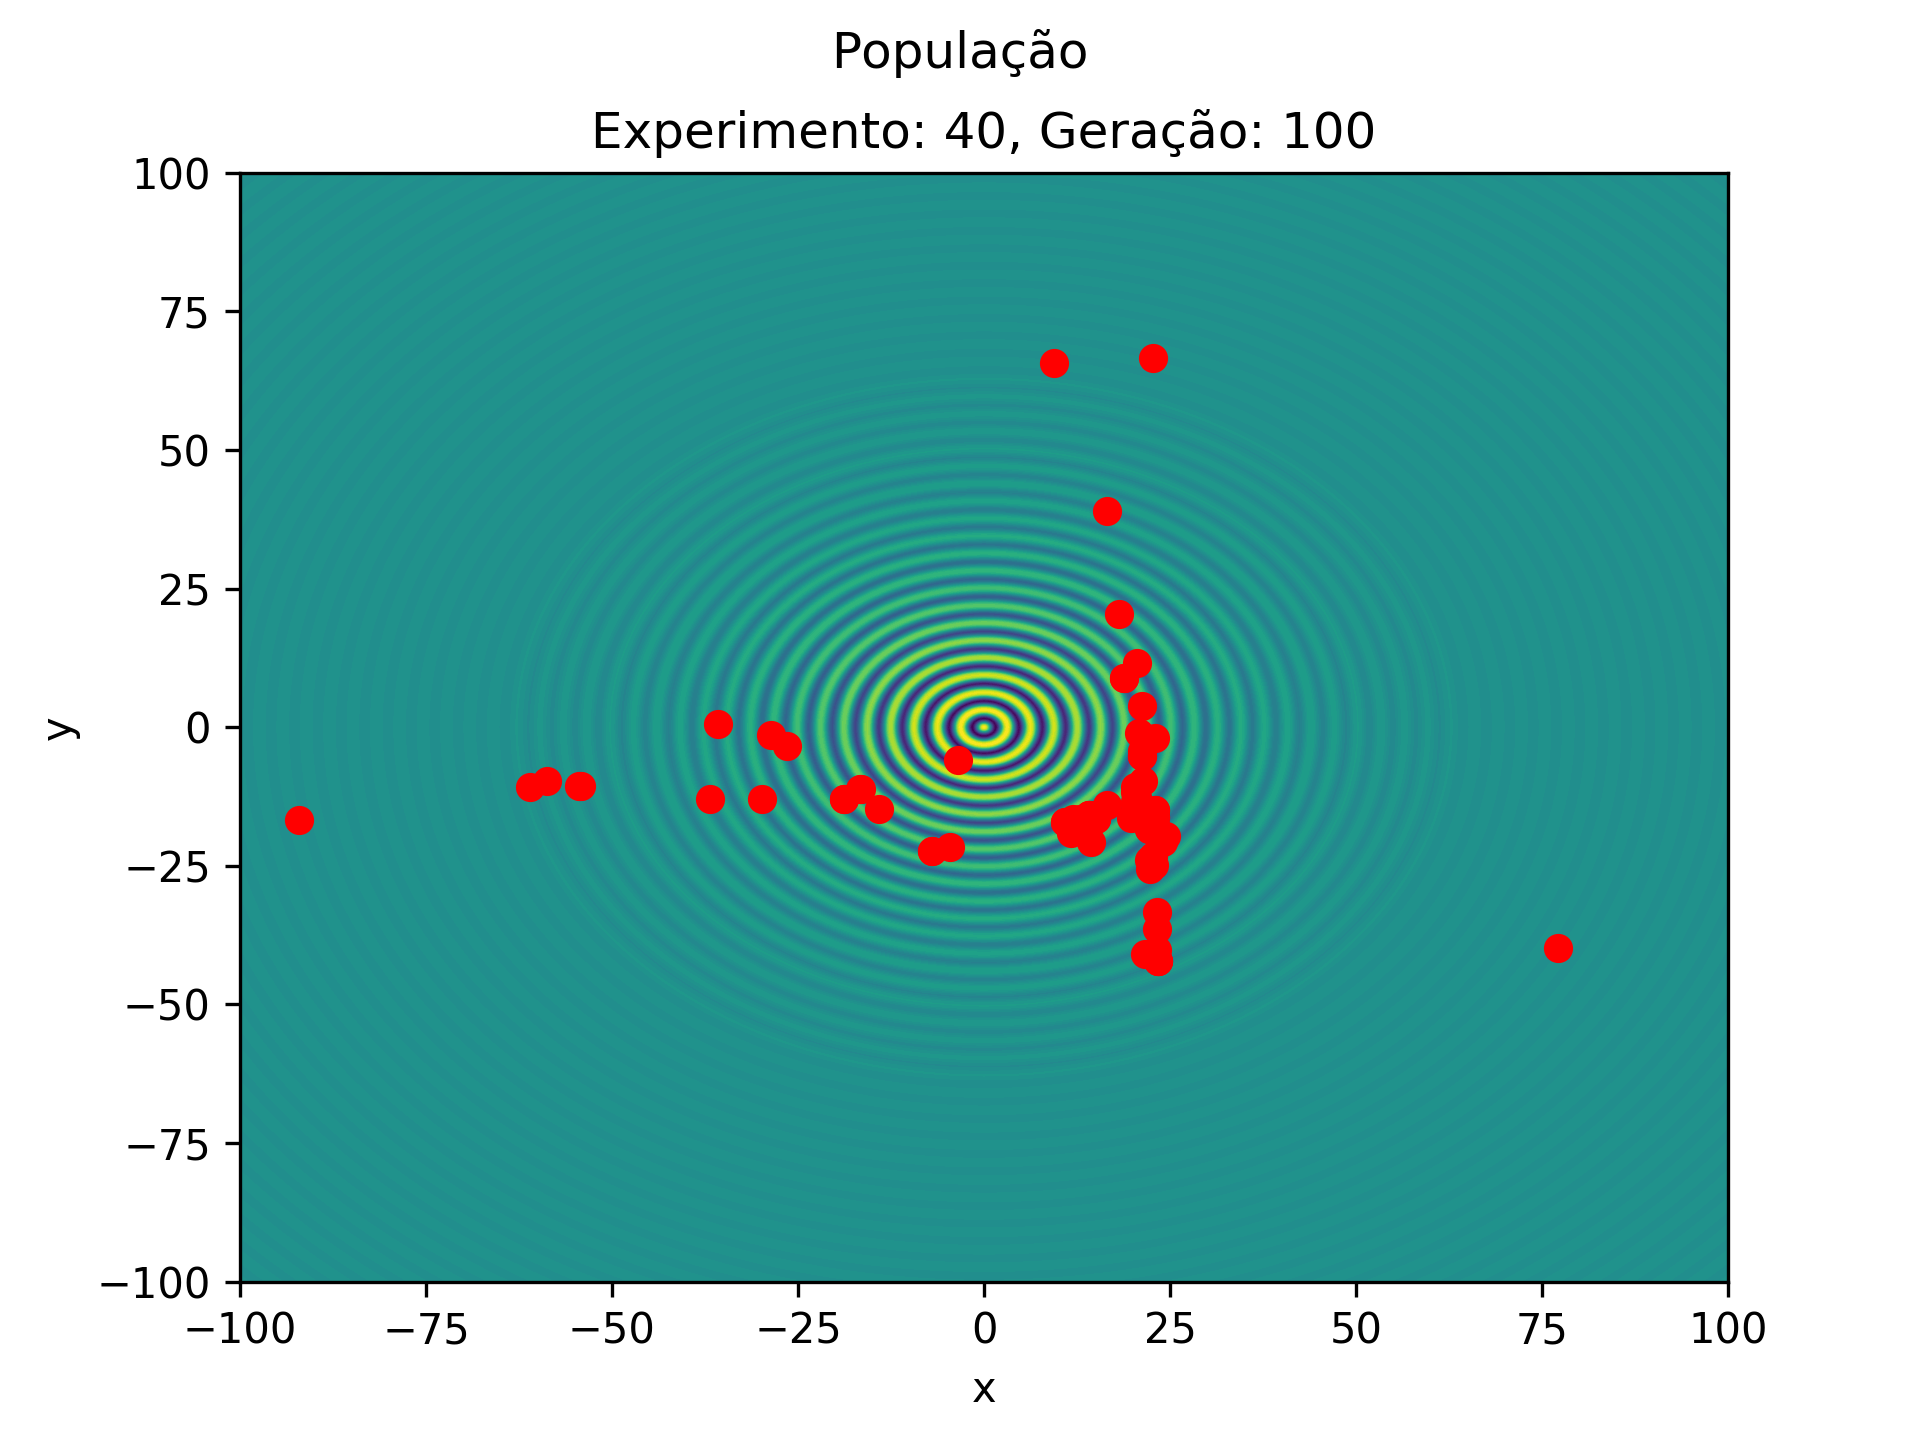
\includegraphics[width=0.9\linewidth]{sec-04/f6_population_gen_100_exp_40.png}
	  \end{subfigure}
	\caption{Populações do experimento 40 nas gerações 1, 10, 50 e 100.}
	\end{figure}